% !TeX root = proyecto.tex

%=========================================================
\chapter{Modelo del Negocio}	
\label{cap:reqSist}


%----------------------------------------------------------
Este capítulo describe a los actores que interactúan con el sistema SICORRE, detallando 
sus responsabilidades, perfil profesional, procesos en los que participan y condiciones 
de uso del sistema. Los actores identificados corresponden al equipo multidisciplinario 
de la Fundación Futuro con Derecho y su personal directivo.

%----------------------------------------------------------
\section{Actores del sistema}

%---------------------------------------------------------
\begin{Usuario}{\hypertarget{A.Directora}{\subsection{Directora}}}{
		Responsable de la supervisión general de la fundación y de la 
		administración del acceso al sistema SICORRE. Actúa como administradora 
		principal en colaboración con la coordinadora.
	}
	\item[Responsabilidades:] \cdtEmpty
	\begin{itemize}
		\item Supervisar la operación general de la Fundación Futuro con Derecho.
		\item Autorizar el alta y baja de usuarios en el sistema en colaboración 
		con la coordinadora.
		\item Revisar y validar el estatus de los expedientes activos de NNA.
		\item Tomar decisiones ejecutivas sobre los casos de restitución de 
		derechos de mayor complejidad o prioridad.
		\item Garantizar el cumplimiento de la normativa de protección de datos 
		de menores (LGDNNA y LGPDPPSO) en el uso del sistema.
		\item Supervisar el trabajo del equipo multidisciplinario y los avances 
		en cada caso.
	\end{itemize}
	
	\item[Perfil:] \cdtEmpty
	\begin{itemize}
		\item Licenciatura en Trabajo Social, Derecho, Psicología o área afín.
		\item Experiencia mínima de 3 años en gestión de organizaciones sociales 
		o fundaciones de atención a menores.
		\item Conocimiento de la normativa mexicana de protección de derechos 
		de niñas, niños y adolescentes (LGDNNA).
		\item Habilidades de liderazgo, toma de decisiones y gestión de equipos 
		multidisciplinarios.
		\item Manejo básico de herramientas digitales y navegadores web.
	\end{itemize}
	
	\item[Procesos en los que participa:] \cdtEmpty
	\begin{itemize}
		\item PR-01 Control de acceso y autenticación.
		\item PR-02 Gestión de usuarios y roles.
		\item PR-03 Gestión de equipos multidisciplinarios.
		\item PR-12 Consulta y búsqueda de información.
		\item PR-13 Control de fechas y calendario de expedientes.
	\end{itemize}
	
	\item[Área:] Dirección General, Fundación Futuro con Derecho.
	\item[Cantidad aproximada:] 1 persona.
	\item[Horario de actividad:] Lunes a viernes de 9:00 a 18:00 horas.
\end{Usuario}

%---------------------------------------------------------
\begin{Usuario}{\hypertarget{A.Coordinadora}{\subsection{Coordinadora}}}{
		Colabora directamente con la directora en la administración del acceso 
		al sistema y en la supervisión operativa del equipo multidisciplinario. 
		Tiene permisos de administración compartidos con la directora.
	}
	\item[Responsabilidades:] \cdtEmpty
	\begin{itemize}
		\item Apoyar a la directora en el control de accesos del personal 
		al sistema.
		\item Coordinar las actividades del equipo multidisciplinario y el 
		seguimiento de los casos activos.
		\item Gestionar la asignación de NNA a los equipos 
		multidisciplinarios correspondientes.
		\item Supervisar el correcto registro de expedientes y valoraciones 
		en el sistema.
		\item Mantener actualizado el catálogo de actores en materia de 
		derechos.
		\item Apoyar en la generación de reportes de avance para la dirección.
	\end{itemize}
	
	\item[Perfil:] \cdtEmpty
	\begin{itemize}
		\item Licenciatura en Trabajo Social, Administración o área afín.
		\item Experiencia mínima de 2 años en coordinación de equipos en 
		organizaciones sociales.
		\item Conocimiento operativo de los procesos de restitución de 
		derechos de NNA.
		\item Habilidades organizativas, comunicación efectiva y manejo 
		de equipos de trabajo.
		\item Manejo intermedio de herramientas digitales y navegadores web.
	\end{itemize}
	
	\item[Procesos en los que participa:] \cdtEmpty
	\begin{itemize}
		\item PR-01 Control de acceso y autenticación.
		\item PR-02 Gestión de usuarios y roles.
		\item PR-03 Gestión de equipos multidisciplinarios.
		\item PR-11 Vinculación de NNA con equipo multidisciplinario.
		\item PR-12 Consulta y búsqueda de información.
		\item PR-13 Control de fechas y calendario de expedientes.
		\item PR-14 Gestión del catálogo de actores en materia de derechos.
	\end{itemize}
	
	\item[Área:] Coordinación Operativa, Fundación Futuro con Derecho.
	\item[Cantidad aproximada:] 1 persona.
	\item[Horario de actividad:] Lunes a viernes de 9:00 a 18:00 horas.
\end{Usuario}

%---------------------------------------------------------
\begin{Usuario}{\hypertarget{A.TrabajadorSocial}{\subsection{Trabajador(a) Social}}}{
		Especialista responsable del primer contacto con el NNA y su entorno 
		familiar. Es el actor principal en el registro inicial de casos, 
		captura de datos del NNA, hecho victimal y tutor, y elaboración 
		de valoraciones sociales.
	}
	\item[Responsabilidades:] \cdtEmpty
	\begin{itemize}
		\item Registrar los datos personales, de ubicación y de 
		vulnerabilidad del NNA conforme al FUD y la caja de herramientas.
		\item Documentar los datos del hecho victimal asociado al caso.
		\item Capturar y mantener actualizados los datos del tutor legal 
		o responsable del NNA.
		\item Abrir y gestionar los expedientes de seguimiento de cada caso.
		\item Registrar sus valoraciones sociales sobre el expediente del NNA.
		\item Identificar y documentar los derechos vulnerados del NNA.
		\item Consultar el catálogo de actores en materia de derechos para 
		articular apoyos disponibles en el municipio del NNA.
		\item Dar seguimiento al calendario de actividades de sus casos activos.
	\end{itemize}
	
	\item[Perfil:] \cdtEmpty
	\begin{itemize}
		\item Licenciatura en Trabajo Social.
		\item Experiencia en atención a poblaciones vulnerables, 
		preferentemente menores de edad.
		\item Conocimiento del FUD y la caja de herramientas para la 
		restitución de derechos de NNA.
		\item Habilidades de empatía, comunicación asertiva y manejo 
		de situaciones de crisis.
		\item Manejo básico de herramientas digitales y formularios en 
		línea.
	\end{itemize}
	
	\item[Procesos en los que participa:] \cdtEmpty
	\begin{itemize}
		\item PR-01 Control de acceso y autenticación.
		\item PR-04 Registro de datos del NNA.
		\item PR-05 Registro del hecho victimal.
		\item PR-06 Registro y gestión del tutor del NNA.
		\item PR-07 Detección de duplicados.
		\item PR-08 Apertura y gestión de expedientes.
		\item PR-09 Registro de valoraciones multidisciplinarias.
		\item PR-10 Registro de derechos vulnerados.
		\item PR-11 Vinculación de NNA con equipo multidisciplinario.
		\item PR-12 Consulta y búsqueda de información.
		\item PR-13 Control de fechas y calendario de expedientes.
		\item PR-15 Vinculación de actores con derechos vulnerados.
	\end{itemize}
	
	\item[Área:] Área Social, Fundación Futuro con Derecho.
	\item[Cantidad aproximada:] 1 persona.
	\item[Horario de actividad:] Lunes a viernes de 9:00 a 18:00 horas, 
	con posibilidad de registro en campo mediante dispositivo móvil 
	con acceso a internet.
\end{Usuario}

%---------------------------------------------------------
\begin{Usuario}{\hypertarget{A.Abogado}{\subsection{Abogado(a)}}}{
		Especialista legal responsable de documentar el estatus jurídico 
		de cada caso, registrar dictámenes legales y dar seguimiento a los 
		derechos vulnerados desde el ámbito del derecho dentro del expediente 
		compartido del equipo multidisciplinario.
	}
	\item[Responsabilidades:] \cdtEmpty
	\begin{itemize}
		\item Registrar valoraciones y dictámenes legales sobre el 
		expediente del NNA.
		\item Documentar las medidas jurídicas sugeridas para la 
		restitución de derechos.
		\item Identificar y registrar los derechos vulnerados desde 
		la perspectiva legal.
		\item Consultar el historial legal de los expedientes activos 
		a su cargo.
		\item Articular con actores en materia de derechos del ámbito 
		jurídico (Procuraduría, DIF, etc.) para la atención de los casos.
		\item Dar seguimiento a las fechas clave de los procesos legales 
		de cada caso.
	\end{itemize}
	
	\item[Perfil:] \cdtEmpty
	\begin{itemize}
		\item Licenciatura en Derecho, con cédula profesional.
		\item Conocimiento de la LGDNNA, Ley General de Víctimas y 
		normativa aplicable a menores de edad en México.
		\item Experiencia en derecho familiar o derechos humanos.
		\item Habilidades analíticas, redacción jurídica y atención 
		al detalle.
		\item Manejo básico de herramientas digitales y navegadores web.
	\end{itemize}
	
	\item[Procesos en los que participa:] \cdtEmpty
	\begin{itemize}
		\item PR-01 Control de acceso y autenticación.
		\item PR-08 Apertura y gestión de expedientes.
		\item PR-09 Registro de valoraciones multidisciplinarias.
		\item PR-10 Registro de derechos vulnerados.
		\item PR-12 Consulta y búsqueda de información.
		\item PR-13 Control de fechas y calendario de expedientes.
		\item PR-15 Vinculación de actores con derechos vulnerados.
	\end{itemize}
	
	\item[Área:] Área Legal, Fundación Futuro con Derecho.
	\item[Cantidad aproximada:] 1 persona.
	\item[Horario de actividad:] Lunes a viernes de 9:00 a 18:00 horas.
\end{Usuario}

%---------------------------------------------------------
\begin{Usuario}{\hypertarget{A.Psicologo}{\subsection{Psicólogo(a)}}}{
		Especialista en salud mental responsable de registrar diagnósticos 
		psicológicos, hallazgos emocionales y medidas de intervención 
		terapéutica para cada NNA dentro del expediente compartido del 
		equipo multidisciplinario.
	}
	\item[Responsabilidades:] \cdtEmpty
	\begin{itemize}
		\item Registrar valoraciones psicológicas, diagnósticos y 
		hallazgos emocionales sobre el expediente del NNA.
		\item Documentar las medidas de intervención terapéutica 
		sugeridas para cada caso.
		\item Identificar y registrar los derechos vulnerados desde 
		la perspectiva de la salud mental.
		\item Consultar el historial psicológico de los expedientes 
		activos a su cargo.
		\item Articular con actores en materia de derechos del ámbito 
		de salud mental disponibles en el municipio del NNA.
		\item Dar seguimiento al calendario de sesiones y actividades 
		terapéuticas programadas.
	\end{itemize}
	
	\item[Perfil:] \cdtEmpty
	\begin{itemize}
		\item Licenciatura en Psicología, con cédula profesional.
		\item Experiencia en psicología clínica infantil o atención 
		a víctimas de violencia.
		\item Conocimiento de técnicas de intervención en crisis y 
		atención a menores en situación de vulnerabilidad.
		\item Habilidades de empatía, escucha activa y redacción 
		de informes clínicos.
		\item Manejo básico de herramientas digitales y navegadores web.
	\end{itemize}
	
	\item[Procesos en los que participa:] \cdtEmpty
	\begin{itemize}
		\item PR-01 Control de acceso y autenticación.
		\item PR-08 Apertura y gestión de expedientes.
		\item PR-09 Registro de valoraciones multidisciplinarias.
		\item PR-10 Registro de derechos vulnerados.
		\item PR-12 Consulta y búsqueda de información.
		\item PR-13 Control de fechas y calendario de expedientes.
		\item PR-15 Vinculación de actores con derechos vulnerados.
	\end{itemize}
	
	\item[Área:] Área de Salud Mental, Fundación Futuro con Derecho.
	\item[Cantidad aproximada:] 1 persona.
	\item[Horario de actividad:] Lunes a viernes de 9:00 a 18:00 horas.
\end{Usuario}

%---------------------------------------------------------
\begin{Usuario}{\hypertarget{A.Medico}{\subsection{Médico(a)}}}{
		Especialista en salud física responsable de documentar el estado 
		de salud del NNA, registrar diagnósticos médicos, enfermedades 
		y actualizar la información de derecho a la salud dentro del 
		expediente compartido del equipo multidisciplinario.
	}
	\item[Responsabilidades:] \cdtEmpty
	\begin{itemize}
		\item Registrar el estado de salud general, diagnósticos médicos 
		y padecimientos del NNA en su expediente.
		\item Documentar las enfermedades crónicas o agudas del NNA y 
		su tutor, indicando si están controladas y el tratamiento en curso.
		\item Registrar las medidas médicas sugeridas para la atención 
		y seguimiento de la salud del NNA.
		\item Identificar y documentar la vulneración del derecho a la 
		salud en los casos que corresponda.
		\item Articular con actores en materia de derechos del ámbito 
		de salud (clínicas, hospitales, ópticas, etc.) disponibles en 
		el municipio del NNA.
		\item Dar seguimiento al calendario de citas y revisiones médicas 
		programadas para cada caso.
	\end{itemize}
	
	\item[Perfil:] \cdtEmpty
	\begin{itemize}
		\item Licenciatura en Medicina, con cédula profesional.
		\item Experiencia en medicina general o pediatría.
		\item Conocimiento de los catálogos de enfermedades (CIE-10 
		o equivalente) y atención a población vulnerable.
		\item Habilidades de diagnóstico clínico, redacción de informes 
		médicos y trabajo interdisciplinario.
		\item Manejo básico de herramientas digitales y navegadores web.
	\end{itemize}
	
	\item[Procesos en los que participa:] \cdtEmpty
	\begin{itemize}
		\item PR-01 Control de acceso y autenticación.
		\item PR-08 Apertura y gestión de expedientes.
		\item PR-09 Registro de valoraciones multidisciplinarias.
		\item PR-10 Registro de derechos vulnerados.
		\item PR-12 Consulta y búsqueda de información.
		\item PR-13 Control de fechas y calendario de expedientes.
		\item PR-15 Vinculación de actores con derechos vulnerados.
		\item PR-16 Gestión de catálogos del sistema.
	\end{itemize}
	
	\item[Área:] Área Médica, Fundación Futuro con Derecho.
	\item[Cantidad aproximada:] 1 persona.
	\item[Horario de actividad:] Lunes a viernes de 9:00 a 18:00 horas.
\end{Usuario}

%---------------------------------------------------------
\section{Términos del Negocio}
\label{sec:terminosDeNegocio}

\cdtInstrucciones{A continuación se definen los términos propios del dominio que aparecen en la especificación del sistema SICORRE.}

\begin{description}
	\item[\textbf{NNA.}]
	Niña, Niño o Adolescente. Persona menor de 18 años beneficiaria
	directa de los servicios de la fundación. Es la entidad central del
	sistema y cada NNA posee un único expediente identificado por su
	CURP.
	
	\item[\textbf{CURP.}]
	Clave Única de Registro de Población. Identificador alfanumérico
	de 18 caracteres asignado por el gobierno mexicano a cada persona.
	Actúa como llave única para el registro de NNA y usuarios en
	SICORRE, impidiendo la creación de expedientes duplicados.
	
	\item[\textbf{FUD (Formato Único de Declaración).}]
	Formato oficial empleado por la Comisión Ejecutiva de Atención a
	Víctimas para registrar a personas en situación de víctima. Sus
	secciones (datos de la víctima, hecho victimizante, datos del tutor,
	tipo de daño, etc.) definen la estructura del módulo de registro de
	NNA en SICORRE.
	
	\item[\textbf{Caja de Herramientas.}]
	Guía práctica para la restitución de derechos de niñas, niños y
	adolescentes emitida por la autoridad competente. Complementa al
	FUD y define los campos de vulnerabilidad, discapacidad, migración y
	pertenencia a comunidades indígenas que el sistema debe capturar.
	
	\item[\textbf{Expediente.}]
	Conjunto de información que documenta el historial completo de un
	caso de restitución de derechos de un NNA. Incluye el folio FUD,
	el estatus del proceso, la prioridad, las valoraciones
	multidisciplinarias y los derechos vulnerados identificados.
	
	\item[\textbf{Hecho Victimal.}]
	Evento delictivo (feminicidio) que origina el estado de orfandad
	del NNA. El registro del hecho victimal incluye el nombre de la
	víctima madre, la fecha del hecho, los datos del expediente jurídico
	y la descripción del delito.
	
	\item[\textbf{Tutor.}]
	Persona adulta — familiar o responsable designado — que tiene a su
	cargo el cuidado y representación legal del NNA ante la fundación.
	Sus datos, domicilio, idioma y padecimientos se registran en el
	sistema.
	
	\item[\textbf{Equipo Multidisciplinario.}]
	Grupo de especialistas (trabajador/a social, abogado/a, psicólogo/a
	y médico/a) que atienden de forma coordinada un mismo conjunto de
	casos. Un NNA se asigna a un equipo, y todos sus integrantes pueden
	visualizar y actualizar el expediente compartido.
	
	\item[\textbf{Valoración.}]
	Registro narrativo que un especialista elabora sobre el expediente
	de un NNA, incluyendo el área de evaluación, los hallazgos y
	dictámenes, las medidas sugeridas y la fecha de la valoración.
	
	\item[\textbf{Derecho Vulnerado.}]
	Derecho específico (a la salud, a la educación, a la identidad,
	etc.) que ha sido transgredido en el caso de un NNA. El sistema
	permite registrar si cada derecho está activamente vulnerado y añadir
	observaciones del equipo.
	
	\item[\textbf{Actor en Materia de Derechos.}]
	Organización gubernamental, no gubernamental o persona física con
	capacidad de participar en la restitución de derechos de los NNA.
	El catálogo de actores se mantiene actualizado con datos de contacto,
	servicios, costos, horarios y ubicación.
	
	\item[\textbf{SEPOMEX.}]
	Servicio Postal Mexicano. Catálogo oficial de códigos postales
	utilizado en SICORRE para normalizar los domicilios de NNA,
	tutores, usuarios y actores, garantizando la correcta asociación de
	colonia, municipio y entidad federativa.
	
	\item[\textbf{INALI.}]
	Instituto Nacional de Lenguas Indígenas. Organismo cuyo catálogo
	oficial de idiomas y variantes dialectales utiliza SICORRE para
	registrar las lenguas maternas del NNA y su tutor.
	
	\item[\textbf{JWT (JSON Web Token).}]
	Mecanismo de autenticación empleado por SICORRE para verificar la
	identidad del usuario en cada petición al servidor, garantizando que
	únicamente el personal autorizado acceda a la información sensible
	de los NNA.
	
	\item[\textbf{Folio FUD.}]
	Número de referencia único asignado a cada expediente dentro del
	sistema, derivado del Formato Único de Declaración oficial. Permite
	relacionar el expediente digital con el trámite físico o
	institucional correspondiente.
	
	\item[\textbf{Rol.}]
	Perfil de permisos asignado a cada usuario del sistema. SICORRE
	define dos roles: \textit{Administrador} (directora y coordinadora,
	con capacidad de gestionar usuarios, equipos y catálogos) y
	\textit{Especialista} (trabajador/a social, abogado/a, psicólogo/a
	y médico/a, con capacidad de registrar y consultar expedientes y
	valoraciones).
\end{description}

%----------------------------------------------------------
\section{Modelo del dominio del problema}
\label{sec:hechosDeNegocio}

El modelo del dominio de SICORRE representa las entidades del negocio y sus
relaciones tal como existen en la operación de la Fundación Futuro con
Derecho. La figura~\ref{fig:DiagramaBDproyecto4} muestra el diagrama entidad-relación
del sistema.

\begin{figure}[htpb!]
	\begin{center}
		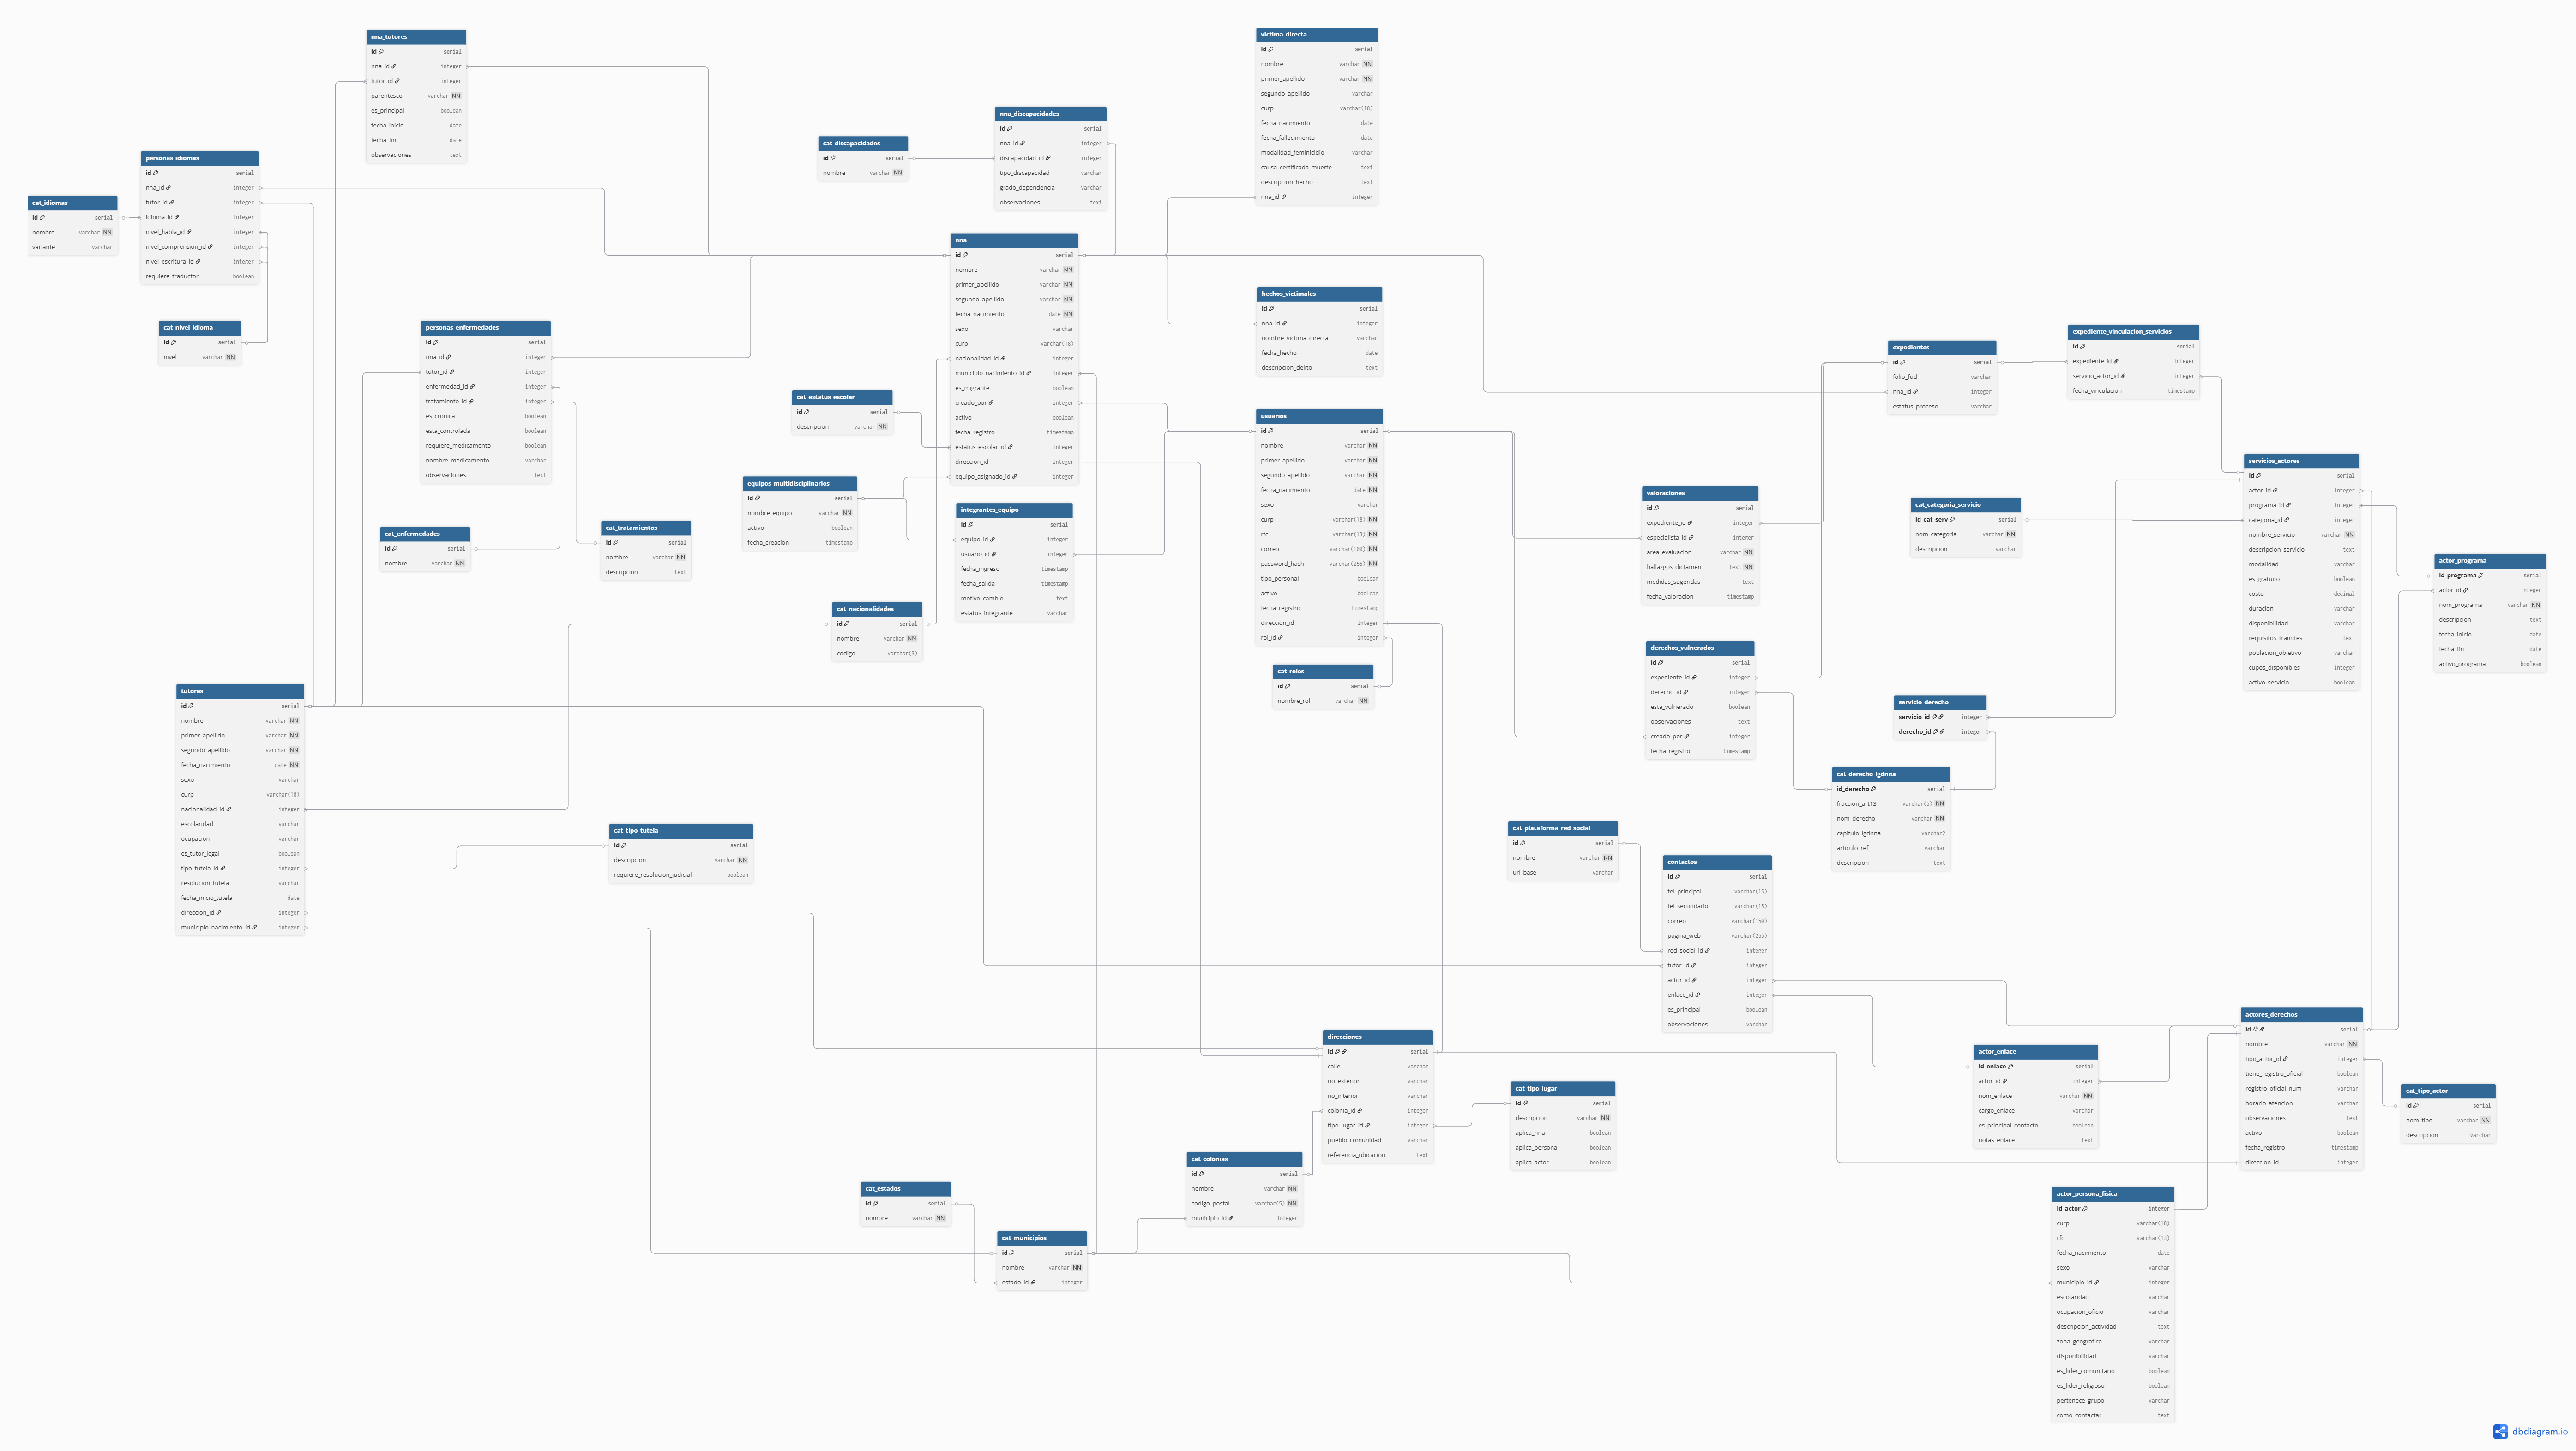
\includegraphics[angle=90,width=.80\textwidth]{images/DiagramaBDproyecto4.png}
		\caption{Modelo del dominio del problema}
		\label{fig:DiagramaBDproyecto4}
	\end{center}
\end{figure}

\clearpage

\begin{cdtEntidad}{CatEstados}{Cat\_Estados}
	\brAttr{id}{Id}{Id}{Identificador único del estado.}{Sí}
	\brAttr{nombre}{Nombre}{Palabra Corta}{Nombre del estado. Debe ser único.}{Sí}
\end{cdtEntidad}

\begin{cdtEntidad}{CatMunicipios}{Cat\_Municipios}
	\brAttr{id}{Id}{Id}{Identificador único del municipio.}{Sí}
	\brAttr{nombre}{Nombre}{Palabra Corta}{Nombre del municipio.}{Sí}
	\brAttr{estadoId}{Estado}{Referencia}{Estado al que pertenece el municipio.}{No}
	\cdtEntityRelSection
	\brRel{\brRelAgregation}{CatEstados}{Un \hyperlink{CatMunicipios}{Cat Municipios} hace referencia a un \hyperlink{CatEstados}{Cat Estados}}
\end{cdtEntidad}

\begin{cdtEntidad}{CatColonias}{Cat\_Colonias}
	\brAttr{id}{Id}{Id}{Identificador único de la colonia.}{Sí}
	\brAttr{nombre}{Nombre}{Palabra Corta}{Nombre de la colonia.}{Sí}
	\brAttr{codigoPostal}{Código Postal}{Palabra Corta}{Código postal de la colonia (5 dígitos).}{Sí}
	\brAttr{municipioId}{Municipio}{Referencia}{Municipio al que pertenece la colonia.}{No}
	\cdtEntityRelSection
	\brRel{\brRelAgregation}{CatMunicipios}{Un \hyperlink{CatColonias}{Cat Colonias} hace referencia a un \hyperlink{CatMunicipios}{Cat Municipios}}
\end{cdtEntidad}

\begin{cdtEntidad}{CatTipoLugar}{Cat\_Tipo\_Lugar}
	\brAttr{id}{Id}{Id}{Identificador único de la entidad.}{Sí}
	\brAttr{descripcion}{Descripcion}{Palabra Corta}{Atributo descripcion de la entidad.}{Sí}
	\brAttr{aplicaNna}{Aplica Nna}{Booleano}{Atributo aplica nna de la entidad.}{No}
	\brAttr{aplicaPersona}{Aplica Persona}{Booleano}{Atributo aplica persona de la entidad.}{No}
	\brAttr{aplicaActor}{Aplica Actor}{Booleano}{Atributo aplica actor de la entidad.}{No}
\end{cdtEntidad}

\begin{cdtEntidad}{CatPlataformaRedSocial}{Cat\_Plataforma\_Red\_Social}
	\brAttr{id}{Id}{Id}{Identificador único de la entidad.}{Sí}
	\brAttr{nombre}{Nombre}{Palabra Corta}{Atributo nombre de la entidad.}{Sí}
	\brAttr{urlBase}{Url Base}{Palabra Corta}{Atributo url base de la entidad.}{No}
\end{cdtEntidad}

\begin{cdtEntidad}{CatRoles}{Cat\_Roles}
	\brAttr{id}{Id}{Id}{Identificador único del rol.}{Sí}
	\brAttr{nombreRol}{Nombre del Rol}{Palabra Corta}{Nombre del rol de usuario. Debe ser único.}{Sí}
\end{cdtEntidad}

\begin{cdtEntidad}{CatNacionalidades}{Cat\_Nacionalidades}
	\brAttr{id}{Id}{Id}{Identificador único de la entidad.}{Sí}
	\brAttr{nombre}{Nombre}{Palabra Corta}{Atributo nombre de la entidad.}{Sí}
\end{cdtEntidad}

\begin{cdtEntidad}{CatEstatusEscolar}{Cat\_Estatus\_Escolar}
	\brAttr{id}{Id}{Id}{Identificador único del estatus escolar.}{Sí}
	\brAttr{descripcion}{Descripción}{Palabra Corta}{Descripción del estatus escolar. Debe ser única.}{Sí}
\end{cdtEntidad}

\begin{cdtEntidad}{CatIdiomas}{Cat\_Idiomas}
	\brAttr{id}{Id}{Id}{Identificador único del idioma.}{Sí}
	\brAttr{nombre}{Nombre}{Palabra Corta}{Nombre del idioma.}{Sí}
	\brAttr{variante}{Variante}{Palabra Corta}{Variante o dialecto del idioma.}{No}
\end{cdtEntidad}

\begin{cdtEntidad}{CatNivelIdioma}{Cat\_Nivel\_Idioma}
	\brAttr{id}{Id}{Id}{Identificador único de la entidad.}{Sí}
	\brAttr{nivel}{Nivel}{Palabra Corta}{Atributo nivel de la entidad.}{Sí}
\end{cdtEntidad}

\begin{cdtEntidad}{CatEnfermedades}{Cat\_Enfermedades}
	\brAttr{id}{Id}{Id}{Identificador único de la enfermedad.}{Sí}
	\brAttr{nombre}{Nombre}{Palabra Corta}{Nombre de la enfermedad.}{Sí}
\end{cdtEntidad}

\begin{cdtEntidad}{CatTratamientos}{Cat\_Tratamientos}
	\brAttr{id}{Id}{Id}{Identificador único de la entidad.}{Sí}
	\brAttr{nombre}{Nombre}{Palabra Corta}{Atributo nombre de la entidad.}{Sí}
	\brAttr{descripcion}{Descripcion}{Texto}{Atributo descripcion de la entidad.}{No}
\end{cdtEntidad}

\begin{cdtEntidad}{CatDiscapacidades}{Cat\_Discapacidades}
	\brAttr{id}{Id}{Id}{Identificador único de la discapacidad.}{Sí}
	\brAttr{nombre}{Nombre}{Palabra Corta}{Nombre de la discapacidad.}{Sí}
\end{cdtEntidad}

\begin{cdtEntidad}{CatTipoActor}{Cat\_Tipo\_Actor}
	\brAttr{id}{Id}{Id}{Identificador único de la entidad.}{Sí}
	\brAttr{nomTipo}{Nom Tipo}{Palabra Corta}{Atributo nom tipo de la entidad.}{Sí}
	\brAttr{descripcion}{Descripcion}{Palabra Corta}{Atributo descripcion de la entidad.}{No}
\end{cdtEntidad}

\begin{cdtEntidad}{CatCategoriaServicio}{Cat\_Categoria\_Servicio}
	\brAttr{idCatServ}{Id Cat Serv}{Id}{Atributo id cat serv de la entidad.}{Sí}
	\brAttr{nomCategoria}{Nom Categoria}{Palabra Corta}{Atributo nom categoria de la entidad.}{Sí}
	\brAttr{descripcion}{Descripcion}{Palabra Corta}{Atributo descripcion de la entidad.}{No}
\end{cdtEntidad}

\begin{cdtEntidad}{CatDerechoLgdnna}{Cat\_Derecho\_Lgdnna}
	\brAttr{idDerecho}{Id Derecho}{Id}{Atributo id derecho de la entidad.}{Sí}
	\brAttr{fraccionArt13}{Fraccion Art13}{Palabra Corta}{Atributo fraccion art13 de la entidad.}{Sí}
	\brAttr{nomDerecho}{Nom Derecho}{Palabra Corta}{Atributo nom derecho de la entidad.}{Sí}
	\brAttr{capituloLgdnna}{Capitulo Lgdnna}{Palabra Corta}{Atributo capitulo lgdnna de la entidad.}{No}
	\brAttr{articuloRef}{Articulo Ref}{Palabra Corta}{Atributo articulo ref de la entidad.}{No}
	\brAttr{descripcion}{Descripcion}{Texto}{Atributo descripcion de la entidad.}{No}
\end{cdtEntidad}

\begin{cdtEntidad}{CatTipoTutela}{Cat\_Tipo\_Tutela}
	\brAttr{id}{Id}{Id}{Identificador único de la entidad.}{Sí}
	\brAttr{descripcion}{Descripcion}{Palabra Corta}{Atributo descripcion de la entidad.}{Sí}
	\brAttr{requiereResolucionJudicial}{Requiere Resolucion Judicial}{Booleano}{Atributo requiere resolucion judicial de la entidad.}{No}
\end{cdtEntidad}

\begin{cdtEntidad}{Direcciones}{Direcciones}
	\brAttr{id}{Id}{Id}{Identificador único de la entidad.}{Sí}
	\brAttr{calle}{Calle}{Palabra Corta}{Atributo calle de la entidad.}{No}
	\brAttr{noExterior}{No Exterior}{Palabra Corta}{Atributo no exterior de la entidad.}{No}
	\brAttr{noInterior}{No Interior}{Palabra Corta}{Atributo no interior de la entidad.}{No}
	\brAttr{coloniaId}{Colonia Id}{Referencia}{Atributo colonia id de la entidad.}{No}
	\brAttr{tipoLugarId}{Tipo Lugar Id}{Referencia}{Atributo tipo lugar id de la entidad.}{No}
	\brAttr{puebloComunidad}{Pueblo Comunidad}{Palabra Corta}{Atributo pueblo comunidad de la entidad.}{No}
	\brAttr{referenciaUbicacion}{Referencia Ubicacion}{Texto}{Atributo referencia ubicacion de la entidad.}{No}
	\cdtEntityRelSection
	\brRel{\brRelAgregation}{CatColonias}{Un \hyperlink{Direcciones}{Direcciones} hace referencia a un \hyperlink{CatColonias}{Cat Colonias}}
	\brRel{\brRelAgregation}{CatTipoLugar}{Un \hyperlink{Direcciones}{Direcciones} hace referencia a un \hyperlink{CatTipoLugar}{Cat Tipo Lugar}}
\end{cdtEntidad}

\begin{cdtEntidad}{Contactos}{Contactos}
	\brAttr{id}{Id}{Id}{Identificador único de la entidad.}{Sí}
	\brAttr{redSocialId}{Red Social Id}{Referencia}{Atributo red social id de la entidad.}{No}
	\brAttr{tutorId}{Tutor Id}{Referencia}{Atributo tutor id de la entidad.}{No}
	\brAttr{actorId}{Actor Id}{Referencia}{Atributo actor id de la entidad.}{No}
	\brAttr{enlaceId}{Enlace Id}{Referencia}{Atributo enlace id de la entidad.}{No}
	\brAttr{esPrincipal}{Es Principal}{Booleano}{Atributo es principal de la entidad.}{No}
	\brAttr{observaciones}{Observaciones}{Palabra Corta}{Atributo observaciones de la entidad.}{No}
	\cdtEntityRelSection
	\brRel{\brRelAgregation}{CatPlataformaRedSocial}{Un \hyperlink{Contactos}{Contactos} hace referencia a un \hyperlink{CatPlataformaRedSocial}{Cat Plataforma Red Social}}
	\brRel{\brRelAgregation}{Tutores}{Un \hyperlink{Contactos}{Contactos} hace referencia a un \hyperlink{Tutores}{Tutores}}
	\brRel{\brRelAgregation}{ActoresDerechos}{Un \hyperlink{Contactos}{Contactos} hace referencia a un \hyperlink{ActoresDerechos}{Actores Derechos}}
	\brRel{\brRelAgregation}{ActorEnlace}{Un \hyperlink{Contactos}{Contactos} hace referencia a un \hyperlink{ActorEnlace}{Actor Enlace}}
\end{cdtEntidad}

\begin{cdtEntidad}{Usuarios}{Usuarios}
	\brAttr{id}{Id}{Id}{Identificador único del usuario.}{Sí}
	\brAttr{nombre}{Nombre}{Palabra Corta}{Nombre o nombres del usuario.}{Sí}
	\brAttr{primerApellido}{Primer Apellido}{Palabra Corta}{Primer apellido del usuario.}{Sí}
	\brAttr{segundoApellido}{Segundo Apellido}{Palabra Corta}{Segundo apellido del usuario.}{Sí}
	\brAttr{fechaNacimiento}{Fecha de Nacimiento}{Fecha}{Fecha de nacimiento del usuario.}{Sí}
	\brAttr{sexo}{Sexo}{Palabra Corta}{Sexo del usuario.}{No}
	\brAttr{curp}{CURP}{Palabra Corta}{CURP del usuario. Debe ser único.}{Sí}
	\brAttr{rfc}{RFC}{Palabra Corta}{RFC del usuario. Debe ser único.}{Sí}
	\brAttr{correo}{Correo}{Palabra Larga}{Correo electrónico del usuario. Debe ser único.}{Sí}
	\brAttr{passwordHash}{Contraseña}{Palabra Larga}{Hash de la contraseña del usuario.}{Sí}
	\brAttr{tipoPersonal}{Tipo de Personal}{Booleano}{Indica el tipo de personal al que pertenece el usuario.}{No}
	\brAttr{activo}{Activo}{Booleano}{Indica si el usuario se encuentra activo en el sistema.}{No}
	\brAttr{fechaRegistro}{Fecha de Registro}{Fecha}{Fecha y hora en que fue registrado el usuario.}{No}
	\brAttr{direccionId}{Dirección}{Referencia}{Dirección del domicilio del usuario.}{No}
	\brAttr{rolId}{Rol}{Referencia}{Rol asignado al usuario dentro del sistema.}{No}
	\cdtEntityRelSection
	\brRel{\brRelComposition}{Direcciones}{Un \hyperlink{Usuarios}{Usuarios} contiene un \hyperlink{Direcciones}{Direcciones}}
	\brRel{\brRelAgregation}{CatRoles}{Un \hyperlink{Usuarios}{Usuarios} hace referencia a un \hyperlink{CatRoles}{Cat Roles}}
\end{cdtEntidad}

\begin{cdtEntidad}{EquiposMultidisciplinarios}{Equipos\_Multidisciplinarios}
	\brAttr{id}{Id}{Id}{Identificador único del equipo multidisciplinario.}{Sí}
	\brAttr{nombreEquipo}{Nombre del Equipo}{Palabra Corta}{Nombre del equipo multidisciplinario.}{Sí}
	\brAttr{activo}{Activo}{Booleano}{Indica si el equipo se encuentra activo.}{No}
	\brAttr{fechaCreacion}{Fecha de Creación}{Fecha}{Fecha y hora en que fue creado el equipo.}{No}
\end{cdtEntidad}

\begin{cdtEntidad}{Tutores}{Tutores}
	\brAttr{id}{Id}{Id}{Identificador único del tutor.}{Sí}
	\brAttr{nombre}{Nombre}{Palabra Corta}{Nombre o nombres del tutor.}{Sí}
	\brAttr{primerApellido}{Primer Apellido}{Palabra Corta}{Primer apellido del tutor.}{Sí}
	\brAttr{segundoApellido}{Segundo Apellido}{Palabra Corta}{Segundo apellido del tutor.}{Sí}
	\brAttr{fechaNacimiento}{Fecha de Nacimiento}{Fecha}{Fecha de nacimiento del tutor.}{Sí}
	\brAttr{sexo}{Sexo}{Palabra Corta}{Sexo del tutor.}{No}
	\brAttr{curp}{CURP}{Palabra Corta}{CURP del tutor. Debe ser único.}{No}
	\brAttr{nacionalidadId}{Nacionalidad Id}{Referencia}{Atributo nacionalidad id de la entidad.}{No}
	\brAttr{escolaridad}{Escolaridad}{Palabra Corta}{Atributo escolaridad de la entidad.}{No}
	\brAttr{ocupacion}{Ocupacion}{Palabra Corta}{Atributo ocupacion de la entidad.}{No}
	\brAttr{esTutorLegal}{Es Tutor Legal}{Booleano}{Atributo es tutor legal de la entidad.}{No}
	\brAttr{tipoTutelaId}{Tipo Tutela Id}{Referencia}{Atributo tipo tutela id de la entidad.}{No}
	\brAttr{resolucionTutela}{Resolucion Tutela}{Palabra Corta}{Atributo resolucion tutela de la entidad.}{No}
	\brAttr{fechaInicioTutela}{Fecha Inicio Tutela}{Fecha}{Atributo fecha inicio tutela de la entidad.}{No}
	\brAttr{direccionId}{Dirección}{Referencia}{Dirección del domicilio del tutor.}{No}
	\brAttr{municipioNacimientoId}{Municipio Nacimiento Id}{Referencia}{Atributo municipio nacimiento id de la entidad.}{No}
	\cdtEntityRelSection
	\brRel{\brRelAgregation}{CatNacionalidades}{Un \hyperlink{Tutores}{Tutores} hace referencia a un \hyperlink{CatNacionalidades}{Cat Nacionalidades}}
	\brRel{\brRelAgregation}{CatMunicipios}{Un \hyperlink{Tutores}{Tutores} hace referencia a un \hyperlink{CatMunicipios}{Cat Municipios}}
	\brRel{\brRelAgregation}{CatTipoTutela}{Un \hyperlink{Tutores}{Tutores} hace referencia a un \hyperlink{CatTipoTutela}{Cat Tipo Tutela}}
	\brRel{\brRelAgregation}{Direcciones}{Un \hyperlink{Tutores}{Tutores} hace referencia a un \hyperlink{Direcciones}{Direcciones}}
\end{cdtEntidad}

\begin{cdtEntidad}{Nna}{Nna}
	\brAttr{id}{Id}{Id}{Identificador único de la entidad.}{Sí}
	\brAttr{nombre}{Nombre}{Palabra Corta}{Atributo nombre de la entidad.}{Sí}
	\brAttr{primerApellido}{Primer Apellido}{Palabra Corta}{Atributo primer apellido de la entidad.}{Sí}
	\brAttr{segundoApellido}{Segundo Apellido}{Palabra Corta}{Atributo segundo apellido de la entidad.}{Sí}
	\brAttr{fechaNacimiento}{Fecha Nacimiento}{Fecha}{Atributo fecha nacimiento de la entidad.}{Sí}
	\brAttr{sexo}{Sexo}{Palabra Corta}{Atributo sexo de la entidad.}{No}
	\brAttr{curp}{Curp}{Palabra Corta}{Atributo curp de la entidad.}{No}
	\brAttr{nacionalidadId}{Nacionalidad Id}{Referencia}{Atributo nacionalidad id de la entidad.}{No}
	\brAttr{municipioNacimientoId}{Municipio Nacimiento Id}{Referencia}{Atributo municipio nacimiento id de la entidad.}{No}
	\brAttr{esMigrante}{Es Migrante}{Booleano}{Atributo es migrante de la entidad.}{No}
	\brAttr{creadoPor}{Creado Por}{Referencia}{Atributo creado por de la entidad.}{No}
	\brAttr{activo}{Activo}{Booleano}{Atributo activo de la entidad.}{No}
	\brAttr{fechaRegistro}{Fecha Registro}{Fecha}{Atributo fecha registro de la entidad.}{No}
	\brAttr{estatusEscolarId}{Estatus Escolar Id}{Referencia}{Atributo estatus escolar id de la entidad.}{No}
	\brAttr{direccionId}{Direccion Id}{Referencia}{Atributo direccion id de la entidad.}{No}
	\brAttr{equipoAsignadoId}{Equipo Asignado Id}{Referencia}{Atributo equipo asignado id de la entidad.}{No}
	\cdtEntityRelSection
	\brRel{\brRelAgregation}{CatNacionalidades}{Un \hyperlink{Nna}{Nna} hace referencia a un \hyperlink{CatNacionalidades}{Cat Nacionalidades}}
	\brRel{\brRelAgregation}{CatMunicipios}{Un \hyperlink{Nna}{Nna} hace referencia a un \hyperlink{CatMunicipios}{Cat Municipios}}
	\brRel{\brRelAgregation}{Usuarios}{Un \hyperlink{Nna}{Nna} hace referencia a un \hyperlink{Usuarios}{Usuarios}}
	\brRel{\brRelAgregation}{CatEstatusEscolar}{Un \hyperlink{Nna}{Nna} hace referencia a un \hyperlink{CatEstatusEscolar}{Cat Estatus Escolar}}
	\brRel{\brRelComposition}{Direcciones}{Un \hyperlink{Nna}{Nna} contiene un \hyperlink{Direcciones}{Direcciones}}
	\brRel{\brRelAgregation}{EquiposMultidisciplinarios}{Un \hyperlink{Nna}{Nna} hace referencia a un \hyperlink{EquiposMultidisciplinarios}{Equipos Multidisciplinarios}}
\end{cdtEntidad}

\begin{cdtEntidad}{VictimaDirecta}{Victima\_Directa}
	\brAttr{id}{Id}{Id}{Identificador único de la entidad.}{Sí}
	\brAttr{nombre}{Nombre}{Palabra Corta}{Atributo nombre de la entidad.}{Sí}
	\brAttr{primerApellido}{Primer Apellido}{Palabra Corta}{Atributo primer apellido de la entidad.}{Sí}
	\brAttr{segundoApellido}{Segundo Apellido}{Palabra Corta}{Atributo segundo apellido de la entidad.}{No}
	\brAttr{curp}{Curp}{Palabra Corta}{Atributo curp de la entidad.}{No}
	\brAttr{fechaNacimiento}{Fecha Nacimiento}{Fecha}{Atributo fecha nacimiento de la entidad.}{No}
	\brAttr{fechaFallecimiento}{Fecha Fallecimiento}{Fecha}{Atributo fecha fallecimiento de la entidad.}{No}
	\brAttr{modalidadFeminicidio}{Modalidad Feminicidio}{Palabra Corta}{Atributo modalidad feminicidio de la entidad.}{No}
	\brAttr{causaCertificadaMuerte}{Causa Certificada Muerte}{Texto}{Atributo causa certificada muerte de la entidad.}{No}
	\brAttr{descripcionHecho}{Descripcion Hecho}{Texto}{Atributo descripcion hecho de la entidad.}{No}
	\brAttr{nnaId}{Nna Id}{Referencia}{Atributo nna id de la entidad.}{No}
	\cdtEntityRelSection
	\brRel{\brRelAgregation}{Nna}{Un \hyperlink{VictimaDirecta}{Victima Directa} hace referencia a un \hyperlink{Nna}{Nna}}
\end{cdtEntidad}

\begin{cdtEntidad}{ActoresDerechos}{Actores\_Derechos}
	\brAttr{id}{Id}{Id}{Identificador único del actor de derechos.}{Sí}
	\brAttr{nombre}{Nombre}{Palabra Corta}{Nombre del actor de derechos.}{Sí}
	\brAttr{tipoActorId}{Tipo Actor Id}{Referencia}{Atributo tipo actor id de la entidad.}{No}
	\brAttr{tieneRegistroOficial}{Tiene Registro Oficial}{Booleano}{Atributo tiene registro oficial de la entidad.}{No}
	\brAttr{registroOficialNum}{Registro Oficial Num}{Palabra Corta}{Atributo registro oficial num de la entidad.}{No}
	\brAttr{horarioAtencion}{Horario Atencion}{Palabra Corta}{Atributo horario atencion de la entidad.}{No}
	\brAttr{observaciones}{Observaciones}{Texto}{Atributo observaciones de la entidad.}{No}
	\brAttr{activo}{Activo}{Booleano}{Atributo activo de la entidad.}{No}
	\brAttr{fechaRegistro}{Fecha Registro}{Fecha}{Atributo fecha registro de la entidad.}{No}
	\brAttr{direccionId}{Dirección}{Referencia}{Dirección del actor de derechos.}{No}
	\cdtEntityRelSection
	\brRel{\brRelAgregation}{CatTipoActor}{Un \hyperlink{ActoresDerechos}{Actores Derechos} hace referencia a un \hyperlink{CatTipoActor}{Cat Tipo Actor}}
	\brRel{\brRelComposition}{Direcciones}{Un \hyperlink{ActoresDerechos}{Actores Derechos} contiene un \hyperlink{Direcciones}{Direcciones}}
\end{cdtEntidad}

\begin{cdtEntidad}{ActorPersonaFisica}{Actor\_Persona\_Fisica}
	\brAttr{idActor}{Id Actor}{Referencia}{Atributo id actor de la entidad.}{Sí}
	\brAttr{curp}{Curp}{Palabra Corta}{Atributo curp de la entidad.}{No}
	\brAttr{fechaNacimiento}{Fecha Nacimiento}{Fecha}{Atributo fecha nacimiento de la entidad.}{No}
	\brAttr{sexo}{Sexo}{Palabra Corta}{Atributo sexo de la entidad.}{No}
	\brAttr{municipioId}{Municipio Id}{Referencia}{Atributo municipio id de la entidad.}{No}
	\brAttr{escolaridad}{Escolaridad}{Palabra Corta}{Atributo escolaridad de la entidad.}{No}
	\brAttr{ocupacionOficio}{Ocupacion Oficio}{Palabra Corta}{Atributo ocupacion oficio de la entidad.}{No}
	\brAttr{descripcionActividad}{Descripcion Actividad}{Texto}{Atributo descripcion actividad de la entidad.}{No}
	\brAttr{zonaGeografica}{Zona Geografica}{Palabra Corta}{Atributo zona geografica de la entidad.}{No}
	\brAttr{disponibilidad}{Disponibilidad}{Palabra Corta}{Atributo disponibilidad de la entidad.}{No}
	\brAttr{esLiderComunitario}{Es Lider Comunitario}{Booleano}{Atributo es lider comunitario de la entidad.}{No}
	\brAttr{esLiderReligioso}{Es Lider Religioso}{Booleano}{Atributo es lider religioso de la entidad.}{No}
	\brAttr{perteneceGrupo}{Pertenece Grupo}{Palabra Corta}{Atributo pertenece grupo de la entidad.}{No}
	\brAttr{comoContactar}{Como Contactar}{Texto}{Atributo como contactar de la entidad.}{No}
	\cdtEntityRelSection
	\brRel{\brRelComposition}{ActoresDerechos}{Un \hyperlink{ActorPersonaFisica}{Actor Persona Fisica} contiene un \hyperlink{ActoresDerechos}{Actores Derechos}}
	\brRel{\brRelAgregation}{CatMunicipios}{Un \hyperlink{ActorPersonaFisica}{Actor Persona Fisica} hace referencia a un \hyperlink{CatMunicipios}{Cat Municipios}}
\end{cdtEntidad}

\begin{cdtEntidad}{ActorEnlace}{Actor\_Enlace}
	\brAttr{idEnlace}{Id Enlace}{Id}{Atributo id enlace de la entidad.}{Sí}
	\brAttr{actorId}{Actor Id}{Referencia}{Atributo actor id de la entidad.}{No}
	\brAttr{nomEnlace}{Nom Enlace}{Palabra Corta}{Atributo nom enlace de la entidad.}{Sí}
	\brAttr{cargoEnlace}{Cargo Enlace}{Palabra Corta}{Atributo cargo enlace de la entidad.}{No}
	\brAttr{esPrincipalContacto}{Es Principal Contacto}{Booleano}{Atributo es principal contacto de la entidad.}{No}
	\brAttr{notasEnlace}{Notas Enlace}{Texto}{Atributo notas enlace de la entidad.}{No}
	\cdtEntityRelSection
	\brRel{\brRelAgregation}{ActoresDerechos}{Un \hyperlink{ActorEnlace}{Actor Enlace} hace referencia a un \hyperlink{ActoresDerechos}{Actores Derechos}}
\end{cdtEntidad}

\begin{cdtEntidad}{ActorPrograma}{Actor\_Programa}
	\brAttr{idPrograma}{Id Programa}{Id}{Atributo id programa de la entidad.}{Sí}
	\brAttr{actorId}{Actor Id}{Referencia}{Atributo actor id de la entidad.}{No}
	\brAttr{nomPrograma}{Nom Programa}{Palabra Corta}{Atributo nom programa de la entidad.}{Sí}
	\brAttr{descripcion}{Descripcion}{Texto}{Atributo descripcion de la entidad.}{No}
	\brAttr{fechaInicio}{Fecha Inicio}{Fecha}{Atributo fecha inicio de la entidad.}{No}
	\brAttr{fechaFin}{Fecha Fin}{Fecha}{Atributo fecha fin de la entidad.}{No}
	\brAttr{activoPrograma}{Activo Programa}{Booleano}{Atributo activo programa de la entidad.}{No}
	\cdtEntityRelSection
	\brRel{\brRelAgregation}{ActoresDerechos}{Un \hyperlink{ActorPrograma}{Actor Programa} hace referencia a un \hyperlink{ActoresDerechos}{Actores Derechos}}
\end{cdtEntidad}

\begin{cdtEntidad}{ServiciosActores}{Servicios\_Actores}
	\brAttr{id}{Id}{Id}{Identificador único del servicio del actor.}{Sí}
	\brAttr{actorId}{Actor}{Referencia}{Actor de derechos que ofrece el servicio.}{No}
	\brAttr{programaId}{Programa Id}{Referencia}{Atributo programa id de la entidad.}{No}
	\brAttr{categoriaId}{Categoria Id}{Referencia}{Atributo categoria id de la entidad.}{No}
	\brAttr{nombreServicio}{Nombre del Servicio}{Palabra Corta}{Nombre del servicio ofrecido por el actor.}{Sí}
	\brAttr{descripcionServicio}{Descripcion Servicio}{Texto}{Atributo descripcion servicio de la entidad.}{No}
	\brAttr{modalidad}{Modalidad}{Palabra Corta}{Atributo modalidad de la entidad.}{No}
	\brAttr{esGratuito}{Es Gratuito}{Booleano}{Indica si el servicio es gratuito.}{No}
	\brAttr{costo}{Costo}{Decimal}{Costo del servicio en caso de no ser gratuito.}{No}
	\brAttr{duracion}{Duración}{Palabra Corta}{Duración estimada del servicio.}{No}
	\brAttr{disponibilidad}{Disponibilidad}{Palabra Corta}{Disponibilidad del servicio.}{No}
	\brAttr{requisitosTramites}{Requisitos y Trámites}{Texto}{Descripción de los requisitos y trámites necesarios para acceder al servicio.}{No}
	\brAttr{poblacionObjetivo}{Poblacion Objetivo}{Palabra Corta}{Atributo poblacion objetivo de la entidad.}{No}
	\brAttr{cuposDisponibles}{Cupos Disponibles}{Entero}{Atributo cupos disponibles de la entidad.}{No}
	\brAttr{activoServicio}{Activo Servicio}{Booleano}{Atributo activo servicio de la entidad.}{No}
	\cdtEntityRelSection
	\brRel{\brRelAgregation}{ActoresDerechos}{Un \hyperlink{ServiciosActores}{Servicios Actores} hace referencia a un \hyperlink{ActoresDerechos}{Actores Derechos}}
	\brRel{\brRelAgregation}{ActorPrograma}{Un \hyperlink{ServiciosActores}{Servicios Actores} hace referencia a un \hyperlink{ActorPrograma}{Actor Programa}}
	\brRel{\brRelAgregation}{CatCategoriaServicio}{Un \hyperlink{ServiciosActores}{Servicios Actores} hace referencia a un \hyperlink{CatCategoriaServicio}{Cat Categoria Servicio}}
\end{cdtEntidad}

\begin{cdtEntidad}{HechosVictimales}{Hechos\_Victimales}
	\brAttr{id}{Id}{Id}{Identificador único del hecho victimal.}{Sí}
	\brAttr{nnaId}{NNA}{Referencia}{NNA al que corresponde el hecho victimal.}{No}
	\brAttr{nombreVictimaDirecta}{Nombre de la Víctima Directa}{Palabra Corta}{Nombre de la víctima directa del hecho.}{No}
	\brAttr{fechaHecho}{Fecha del Hecho}{Fecha}{Fecha en que ocurrió el hecho victimal.}{No}
	\brAttr{descripcionDelito}{Descripción del Delito}{Texto}{Descripción del delito o hecho victimal ocurrido.}{No}
	\cdtEntityRelSection
	\brRel{\brRelAgregation}{Nna}{Un \hyperlink{HechosVictimales}{Hechos Victimales} hace referencia a un \hyperlink{Nna}{Nna}}
\end{cdtEntidad}

\begin{cdtEntidad}{Expedientes}{Expedientes}
	\brAttr{id}{Id}{Id}{Identificador único del expediente.}{Sí}
	\brAttr{folioFud}{Folio FUD}{Palabra Corta}{Folio único de identificación del expediente. Debe ser único.}{No}
	\brAttr{nnaId}{NNA}{Referencia}{NNA al que pertenece el expediente.}{No}
	\brAttr{estatusProceso}{Estatus del Proceso}{Palabra Corta}{Estatus actual del proceso del expediente.}{No}
	\cdtEntityRelSection
	\brRel{\brRelAgregation}{Nna}{Un \hyperlink{Expedientes}{Expedientes} hace referencia a un \hyperlink{Nna}{Nna}}
\end{cdtEntidad}

\begin{cdtEntidad}{Valoraciones}{Valoraciones}
	\brAttr{id}{Id}{Id}{Identificador único de la valoración.}{Sí}
	\brAttr{expedienteId}{Expediente}{Referencia}{Expediente al que corresponde la valoración.}{No}
	\brAttr{especialistaId}{Especialista}{Referencia}{Usuario especialista que realizó la valoración.}{No}
	\brAttr{areaEvaluacion}{Área de Evaluación}{Palabra Corta}{Área en la que se realizó la evaluación.}{Sí}
	\brAttr{hallazgosDictamen}{Hallazgos y Dictamen}{Texto}{Descripción de los hallazgos y dictamen de la valoración.}{Sí}
	\brAttr{medidasSugeridas}{Medidas Sugeridas}{Texto}{Medidas sugeridas a partir de la valoración.}{No}
	\brAttr{fechaValoracion}{Fecha de Valoración}{Fecha}{Fecha y hora en que se realizó la valoración.}{No}
	\cdtEntityRelSection
	\brRel{\brRelAgregation}{Expedientes}{Un \hyperlink{Valoraciones}{Valoraciones} hace referencia a un \hyperlink{Expedientes}{Expedientes}}
	\brRel{\brRelAgregation}{Usuarios}{Un \hyperlink{Valoraciones}{Valoraciones} hace referencia a un \hyperlink{Usuarios}{Usuarios}}
\end{cdtEntidad}

\begin{cdtEntidad}{DerechosVulnerados}{Derechos\_Vulnerados}
	\brAttr{id}{Id}{Id}{Identificador único del derecho vulnerado.}{Sí}
	\brAttr{expedienteId}{Expediente}{Referencia}{Expediente al que corresponde el derecho vulnerado.}{No}
	\brAttr{derechoId}{Derecho Id}{Referencia}{Atributo derecho id de la entidad.}{No}
	\brAttr{estaVulnerado}{Está Vulnerado}{Booleano}{Indica si el derecho se encuentra vulnerado.}{No}
	\brAttr{observaciones}{Observaciones}{Texto}{Observaciones sobre el derecho vulnerado.}{No}
	\brAttr{creadoPor}{Creado Por}{Referencia}{Usuario que registró el derecho vulnerado.}{No}
	\brAttr{fechaRegistro}{Fecha de Registro}{Fecha}{Fecha y hora en que fue registrado el derecho vulnerado.}{No}
	\cdtEntityRelSection
	\brRel{\brRelAgregation}{Expedientes}{Un \hyperlink{DerechosVulnerados}{Derechos Vulnerados} hace referencia a un \hyperlink{Expedientes}{Expedientes}}
	\brRel{\brRelAgregation}{CatDerechoLgdnna}{Un \hyperlink{DerechosVulnerados}{Derechos Vulnerados} hace referencia a un \hyperlink{CatDerechoLgdnna}{Cat Derecho Lgdnna}}
	\brRel{\brRelAgregation}{Usuarios}{Un \hyperlink{DerechosVulnerados}{Derechos Vulnerados} hace referencia a un \hyperlink{Usuarios}{Usuarios}}
\end{cdtEntidad}

\begin{cdtEntidad}{NnaTutores}{Nna\_Tutores}
	\brAttr{id}{Id}{Id}{Identificador único de la entidad.}{Sí}
	\brAttr{nnaId}{Nna Id}{Referencia}{Atributo nna id de la entidad.}{No}
	\brAttr{tutorId}{Tutor Id}{Referencia}{Atributo tutor id de la entidad.}{No}
	\brAttr{parentesco}{Parentesco}{Palabra Corta}{Atributo parentesco de la entidad.}{Sí}
	\brAttr{esPrincipal}{Es Principal}{Booleano}{Atributo es principal de la entidad.}{No}
	\brAttr{fechaInicio}{Fecha Inicio}{Fecha}{Atributo fecha inicio de la entidad.}{No}
	\brAttr{fechaFin}{Fecha Fin}{Fecha}{Atributo fecha fin de la entidad.}{No}
	\brAttr{observaciones}{Observaciones}{Texto}{Atributo observaciones de la entidad.}{No}
	\cdtEntityRelSection
	\brRel{\brRelAgregation}{Nna}{Un \hyperlink{NnaTutores}{Nna Tutores} hace referencia a un \hyperlink{Nna}{Nna}}
	\brRel{\brRelAgregation}{Tutores}{Un \hyperlink{NnaTutores}{Nna Tutores} hace referencia a un \hyperlink{Tutores}{Tutores}}
\end{cdtEntidad}

\begin{cdtEntidad}{IntegrantesEquipo}{Integrantes\_Equipo}
	\brAttr{id}{Id}{Id}{Identificador único del registro de integrante.}{Sí}
	\brAttr{equipoId}{Equipo}{Referencia}{Equipo multidisciplinario al que pertenece el integrante.}{No}
	\brAttr{usuarioId}{Usuario}{Referencia}{Usuario que forma parte del equipo.}{No}
	\brAttr{fechaIngreso}{Fecha de Ingreso}{Fecha}{Fecha y hora en que el usuario ingresó al equipo.}{No}
	\brAttr{fechaSalida}{Fecha de Salida}{Fecha}{Fecha y hora en que el usuario salió del equipo.}{No}
	\brAttr{motivoCambio}{Motivo de Cambio}{Texto}{Descripción del motivo por el cual se realizó un cambio en el equipo.}{No}
	\brAttr{estatusIntegrante}{Estatus del Integrante}{Palabra Corta}{Estatus actual del integrante dentro del equipo.}{No}
	\cdtEntityRelSection
	\brRel{\brRelAgregation}{EquiposMultidisciplinarios}{Un \hyperlink{IntegrantesEquipo}{Integrantes Equipo} hace referencia a un \hyperlink{EquiposMultidisciplinarios}{Equipos Multidisciplinarios}}
	\brRel{\brRelAgregation}{Usuarios}{Un \hyperlink{IntegrantesEquipo}{Integrantes Equipo} hace referencia a un \hyperlink{Usuarios}{Usuarios}}
\end{cdtEntidad}

\begin{cdtEntidad}{PersonasEnfermedades}{Personas\_Enfermedades}
	\brAttr{id}{Id}{Id}{Identificador único de la entidad.}{Sí}
	\brAttr{nnaId}{Nna Id}{Referencia}{Atributo nna id de la entidad.}{No}
	\brAttr{tutorId}{Tutor Id}{Referencia}{Atributo tutor id de la entidad.}{No}
	\brAttr{enfermedadId}{Enfermedad Id}{Referencia}{Atributo enfermedad id de la entidad.}{No}
	\brAttr{tratamientoId}{Tratamiento Id}{Referencia}{Atributo tratamiento id de la entidad.}{No}
	\brAttr{esCronica}{Es Cronica}{Booleano}{Atributo es cronica de la entidad.}{No}
	\brAttr{estaControlada}{Esta Controlada}{Booleano}{Atributo esta controlada de la entidad.}{No}
	\brAttr{requiereMedicamento}{Requiere Medicamento}{Booleano}{Atributo requiere medicamento de la entidad.}{No}
	\brAttr{nombreMedicamento}{Nombre Medicamento}{Palabra Corta}{Atributo nombre medicamento de la entidad.}{No}
	\brAttr{observaciones}{Observaciones}{Texto}{Atributo observaciones de la entidad.}{No}
	\cdtEntityRelSection
	\brRel{\brRelAgregation}{Nna}{Un \hyperlink{PersonasEnfermedades}{Personas Enfermedades} hace referencia a un \hyperlink{Nna}{Nna}}
	\brRel{\brRelAgregation}{Tutores}{Un \hyperlink{PersonasEnfermedades}{Personas Enfermedades} hace referencia a un \hyperlink{Tutores}{Tutores}}
	\brRel{\brRelAgregation}{CatEnfermedades}{Un \hyperlink{PersonasEnfermedades}{Personas Enfermedades} hace referencia a un \hyperlink{CatEnfermedades}{Cat Enfermedades}}
	\brRel{\brRelAgregation}{CatTratamientos}{Un \hyperlink{PersonasEnfermedades}{Personas Enfermedades} hace referencia a un \hyperlink{CatTratamientos}{Cat Tratamientos}}
\end{cdtEntidad}

\begin{cdtEntidad}{PersonasIdiomas}{Personas\_Idiomas}
	\brAttr{id}{Id}{Id}{Identificador único de la entidad.}{Sí}
	\brAttr{nnaId}{Nna Id}{Referencia}{Atributo nna id de la entidad.}{No}
	\brAttr{tutorId}{Tutor Id}{Referencia}{Atributo tutor id de la entidad.}{No}
	\brAttr{idiomaId}{Idioma Id}{Referencia}{Atributo idioma id de la entidad.}{No}
	\brAttr{nivelHablaId}{Nivel Habla Id}{Referencia}{Atributo nivel habla id de la entidad.}{No}
	\brAttr{nivelComprensionId}{Nivel Comprension Id}{Referencia}{Atributo nivel comprension id de la entidad.}{No}
	\brAttr{nivelEscrituraId}{Nivel Escritura Id}{Referencia}{Atributo nivel escritura id de la entidad.}{No}
	\brAttr{requiereTraductor}{Requiere Traductor}{Booleano}{Atributo requiere traductor de la entidad.}{No}
	\cdtEntityRelSection
	\brRel{\brRelAgregation}{Nna}{Un \hyperlink{PersonasIdiomas}{Personas Idiomas} hace referencia a un \hyperlink{Nna}{Nna}}
	\brRel{\brRelAgregation}{Tutores}{Un \hyperlink{PersonasIdiomas}{Personas Idiomas} hace referencia a un \hyperlink{Tutores}{Tutores}}
	\brRel{\brRelAgregation}{CatIdiomas}{Un \hyperlink{PersonasIdiomas}{Personas Idiomas} hace referencia a un \hyperlink{CatIdiomas}{Cat Idiomas}}
	\brRel{\brRelAgregation}{CatNivelIdioma}{Un \hyperlink{PersonasIdiomas}{Personas Idiomas} hace referencia a un \hyperlink{CatNivelIdioma}{Cat Nivel Idioma}}
	\brRel{\brRelAgregation}{CatNivelIdioma}{Un \hyperlink{PersonasIdiomas}{Personas Idiomas} hace referencia a un \hyperlink{CatNivelIdioma}{Cat Nivel Idioma}}
	\brRel{\brRelAgregation}{CatNivelIdioma}{Un \hyperlink{PersonasIdiomas}{Personas Idiomas} hace referencia a un \hyperlink{CatNivelIdioma}{Cat Nivel Idioma}}
\end{cdtEntidad}

\begin{cdtEntidad}{NnaDiscapacidades}{Nna\_Discapacidades}
	\brAttr{id}{Id}{Id}{Identificador único de la entidad.}{Sí}
	\brAttr{nnaId}{Nna Id}{Referencia}{Atributo nna id de la entidad.}{No}
	\brAttr{discapacidadId}{Discapacidad Id}{Referencia}{Atributo discapacidad id de la entidad.}{No}
	\brAttr{tipoDiscapacidad}{Tipo Discapacidad}{Palabra Corta}{Atributo tipo discapacidad de la entidad.}{No}
	\brAttr{gradoDependencia}{Grado Dependencia}{Palabra Corta}{Atributo grado dependencia de la entidad.}{No}
	\brAttr{observaciones}{Observaciones}{Texto}{Atributo observaciones de la entidad.}{No}
	\cdtEntityRelSection
	\brRel{\brRelAgregation}{Nna}{Un \hyperlink{NnaDiscapacidades}{Nna Discapacidades} hace referencia a un \hyperlink{Nna}{Nna}}
	\brRel{\brRelAgregation}{CatDiscapacidades}{Un \hyperlink{NnaDiscapacidades}{Nna Discapacidades} hace referencia a un \hyperlink{CatDiscapacidades}{Cat Discapacidades}}
\end{cdtEntidad}

\begin{cdtEntidad}{ServicioDerecho}{Servicio\_Derecho}
	\brAttr{servicioId}{Servicio Id}{Referencia}{Atributo servicio id de la entidad.}{No}
	\brAttr{derechoId}{Derecho Id}{Referencia}{Atributo derecho id de la entidad.}{No}
		\cdtEntityRelSection
	\brRel{\brRelAgregation}{ServiciosActores}{Un \hyperlink{ServicioDerecho}{Servicio Derecho} hace referencia a un \hyperlink{ServiciosActores}{Servicios Actores}}
	\brRel{\brRelAgregation}{CatDerechoLgdnna}{Un \hyperlink{ServicioDerecho}{Servicio Derecho} hace referencia a un \hyperlink{CatDerechoLgdnna}{Cat Derecho Lgdnna}}
\end{cdtEntidad}

\begin{cdtEntidad}{ExpedienteVinculacionServicios}{Expediente\_Vinculacion\_Servicios}
	\brAttr{id}{Id}{Id}{Identificador único del registro de vinculación.}{Sí}
	\brAttr{expedienteId}{Expediente}{Referencia}{Expediente vinculado al servicio.}{No}
	\brAttr{servicioActorId}{Servicio del Actor}{Referencia}{Servicio del actor de derechos al que se vincula el expediente.}{No}
	\brAttr{fechaVinculacion}{Fecha de Vinculación}{Fecha}{Fecha y hora en que se realizó la vinculación.}{No}
	\cdtEntityRelSection
	\brRel{\brRelAgregation}{Expedientes}{Un \hyperlink{ExpedienteVinculacionServicios}{Expediente Vinculacion Servicios} hace referencia a un \hyperlink{Expedientes}{Expedientes}}
	\brRel{\brRelAgregation}{ServiciosActores}{Un \hyperlink{ExpedienteVinculacionServicios}{Expediente Vinculacion Servicios} hace referencia a un \hyperlink{ServiciosActores}{Servicios Actores}}
\end{cdtEntidad}


